% !TEX root = main.tex

% TODO:
% REMARK:

\section{Background Estimation}
\label{sec:BkgEst}

	According to the simulation, the events of interests occupy diminant ratio under signal region selection(includes $\chi^2_{min}$, MVA-A, MVA-B strategy), but also about 4$\sim$6 \% of events which came from non-$t\bar{t}$ background are collected. Even though the selected events are under high signal purity, the randomly combined background events would contaminate the final measurement of asymmetry. In fact, the minority of background may still dilute the calculating results of $A'_{cp}$ critically in this precision measurement analysis. Thus, the background study should be attached importance to. The $A'_{cp}$ value of $t\bar{t}$ would be extracted, at the same time, backgrounds' contribution would be cast aside.

	It is a common and usual way to estimate background in data by using simulation samples. It depends more on the theoretical modeling and detector simulation with simulation sample. The background in simulation cannot be quite close to real data perfectly. This situation would disorder the asymmetry measurement eventually. It is suggested that in many high energy experiments' analysis to directly acquire background from real data. Therefore, the data-driven way is applied.
	
	In this analysis, it is found that the $M_{lb}$ variable shows really difference between signal and background in shape(Fig.\ref{BkgEst:fig:SR_sigbkg_Mlbshape}). Thus, with the diverse shape, there is an advantage to discern signal and background and then seperate them with template fit.

	\begin{figure}[H]
		\centering
			\subfigure[$\chi^2_{min}$, mu-ch]{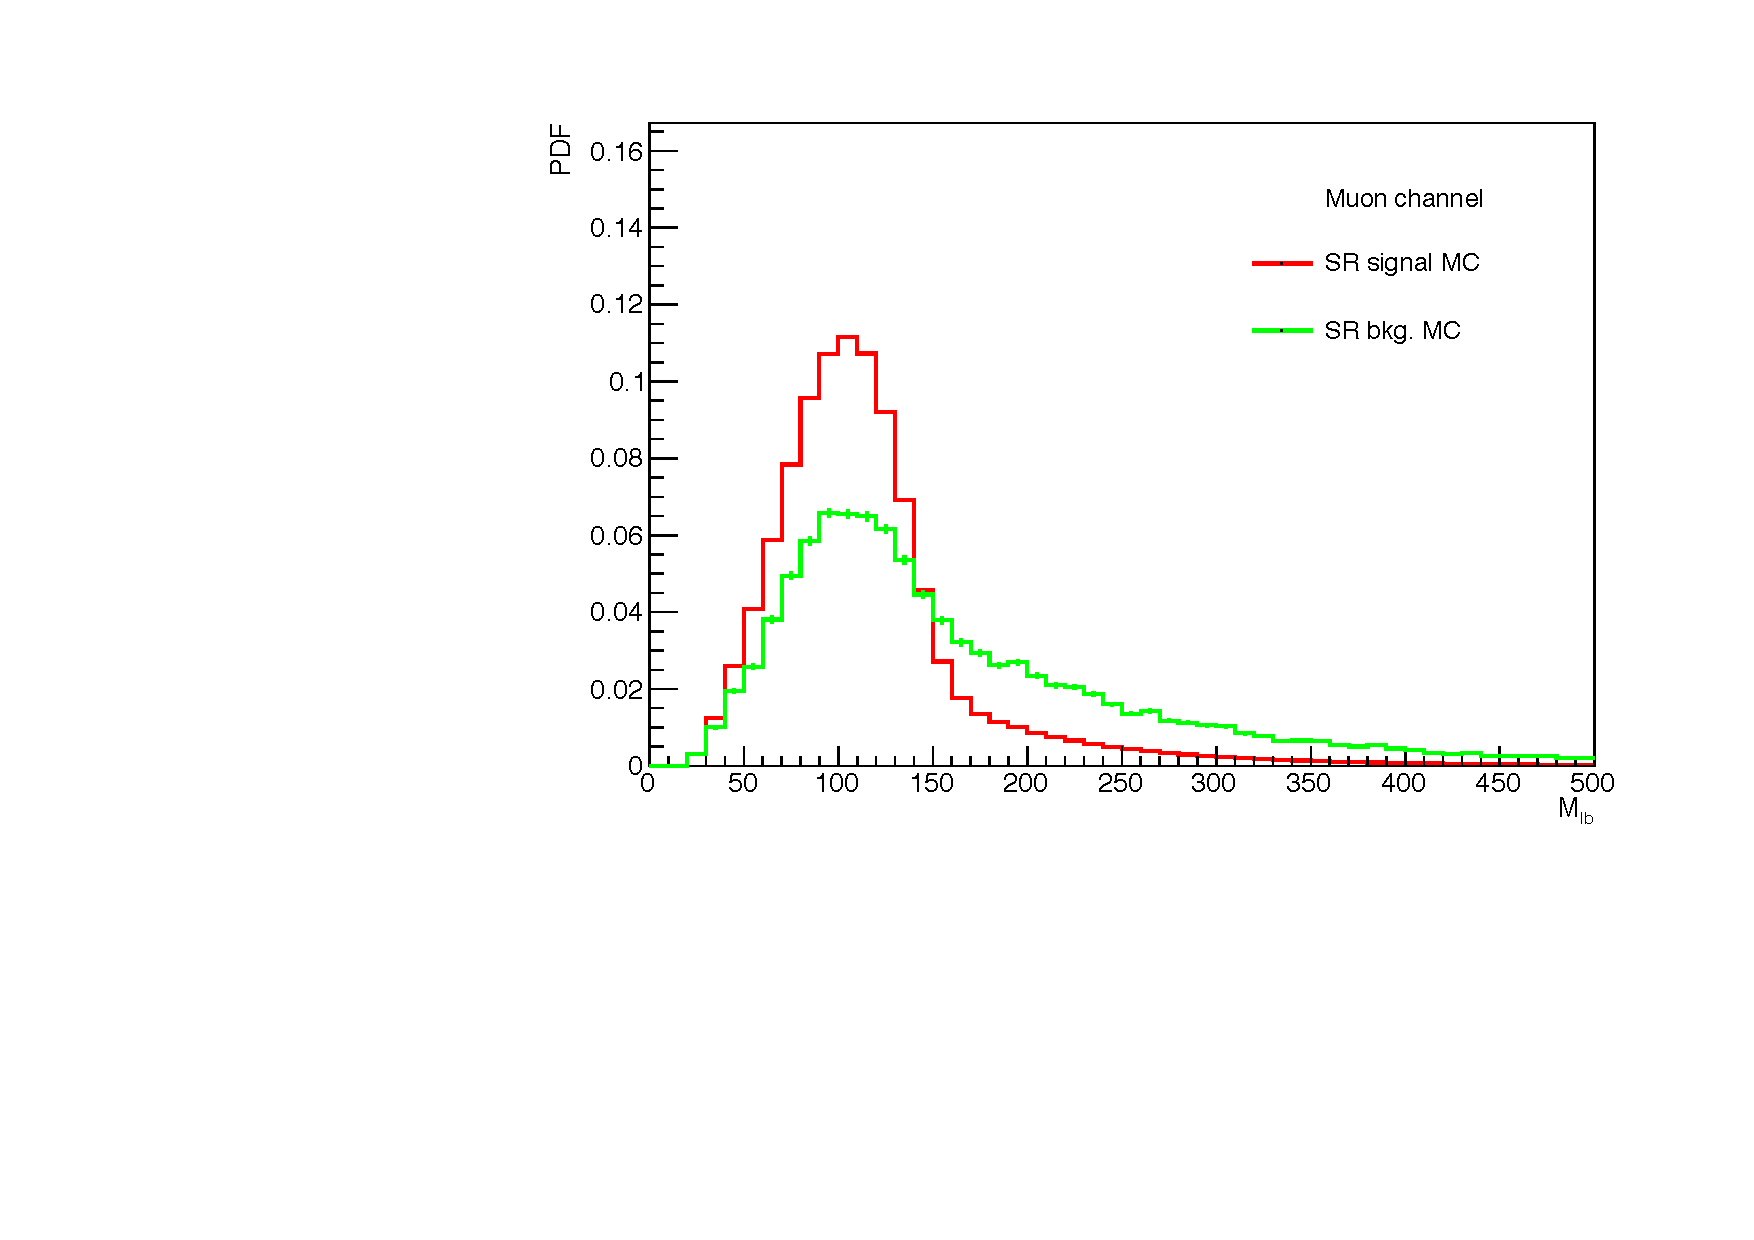
\includegraphics[width=0.45\textwidth]{Figures/BackgroundEstimation/chi2_SR_sig_bkg_shape_mu.pdf}}
			\subfigure[$\chi^2_{min}$, el-ch]{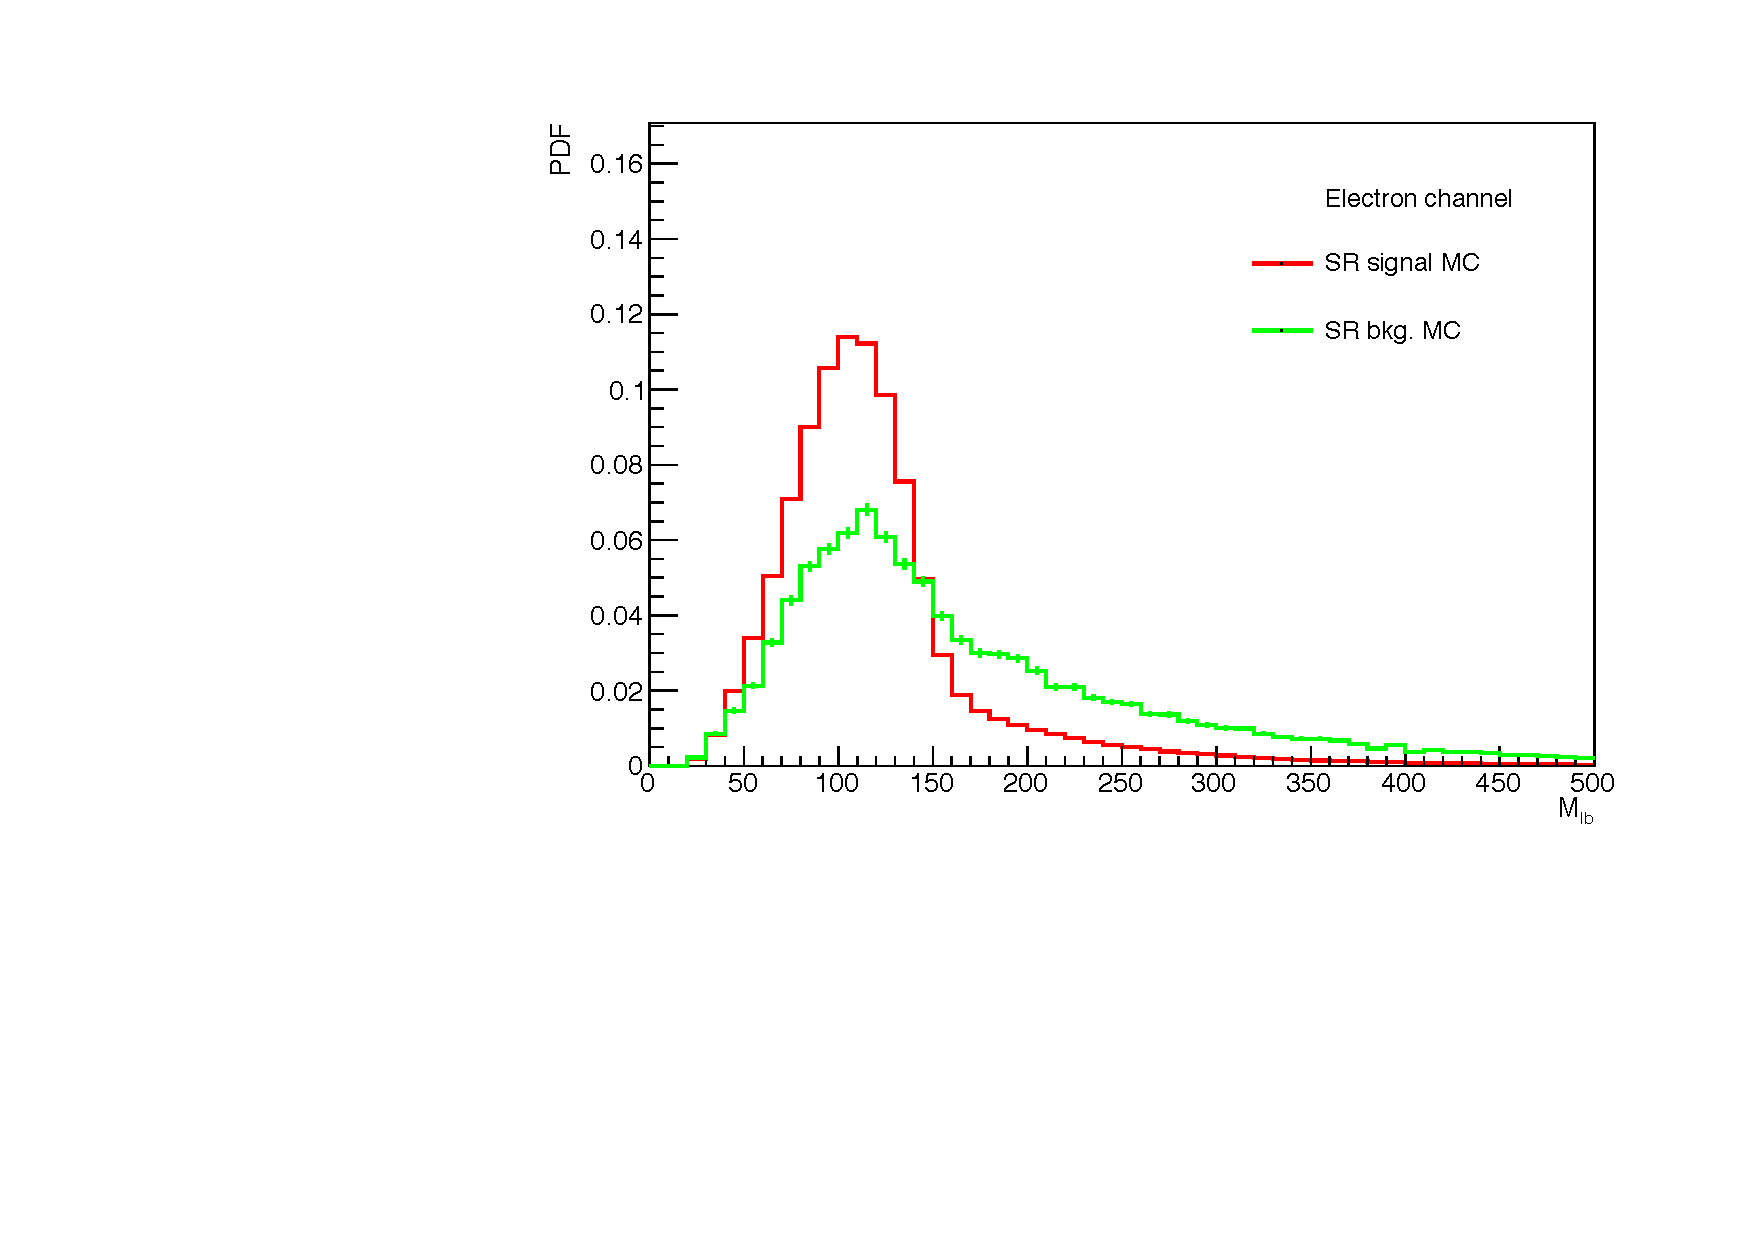
\includegraphics[width=0.45\textwidth]{Figures/BackgroundEstimation/chi2_SR_sig_bkg_shape_el.pdf}}\\
		\end{figure}
		\FloatBarrier
		\begin{figure}[H]
		\centering
			\subfigure[MVA(20 variables, MLP), mu-ch]{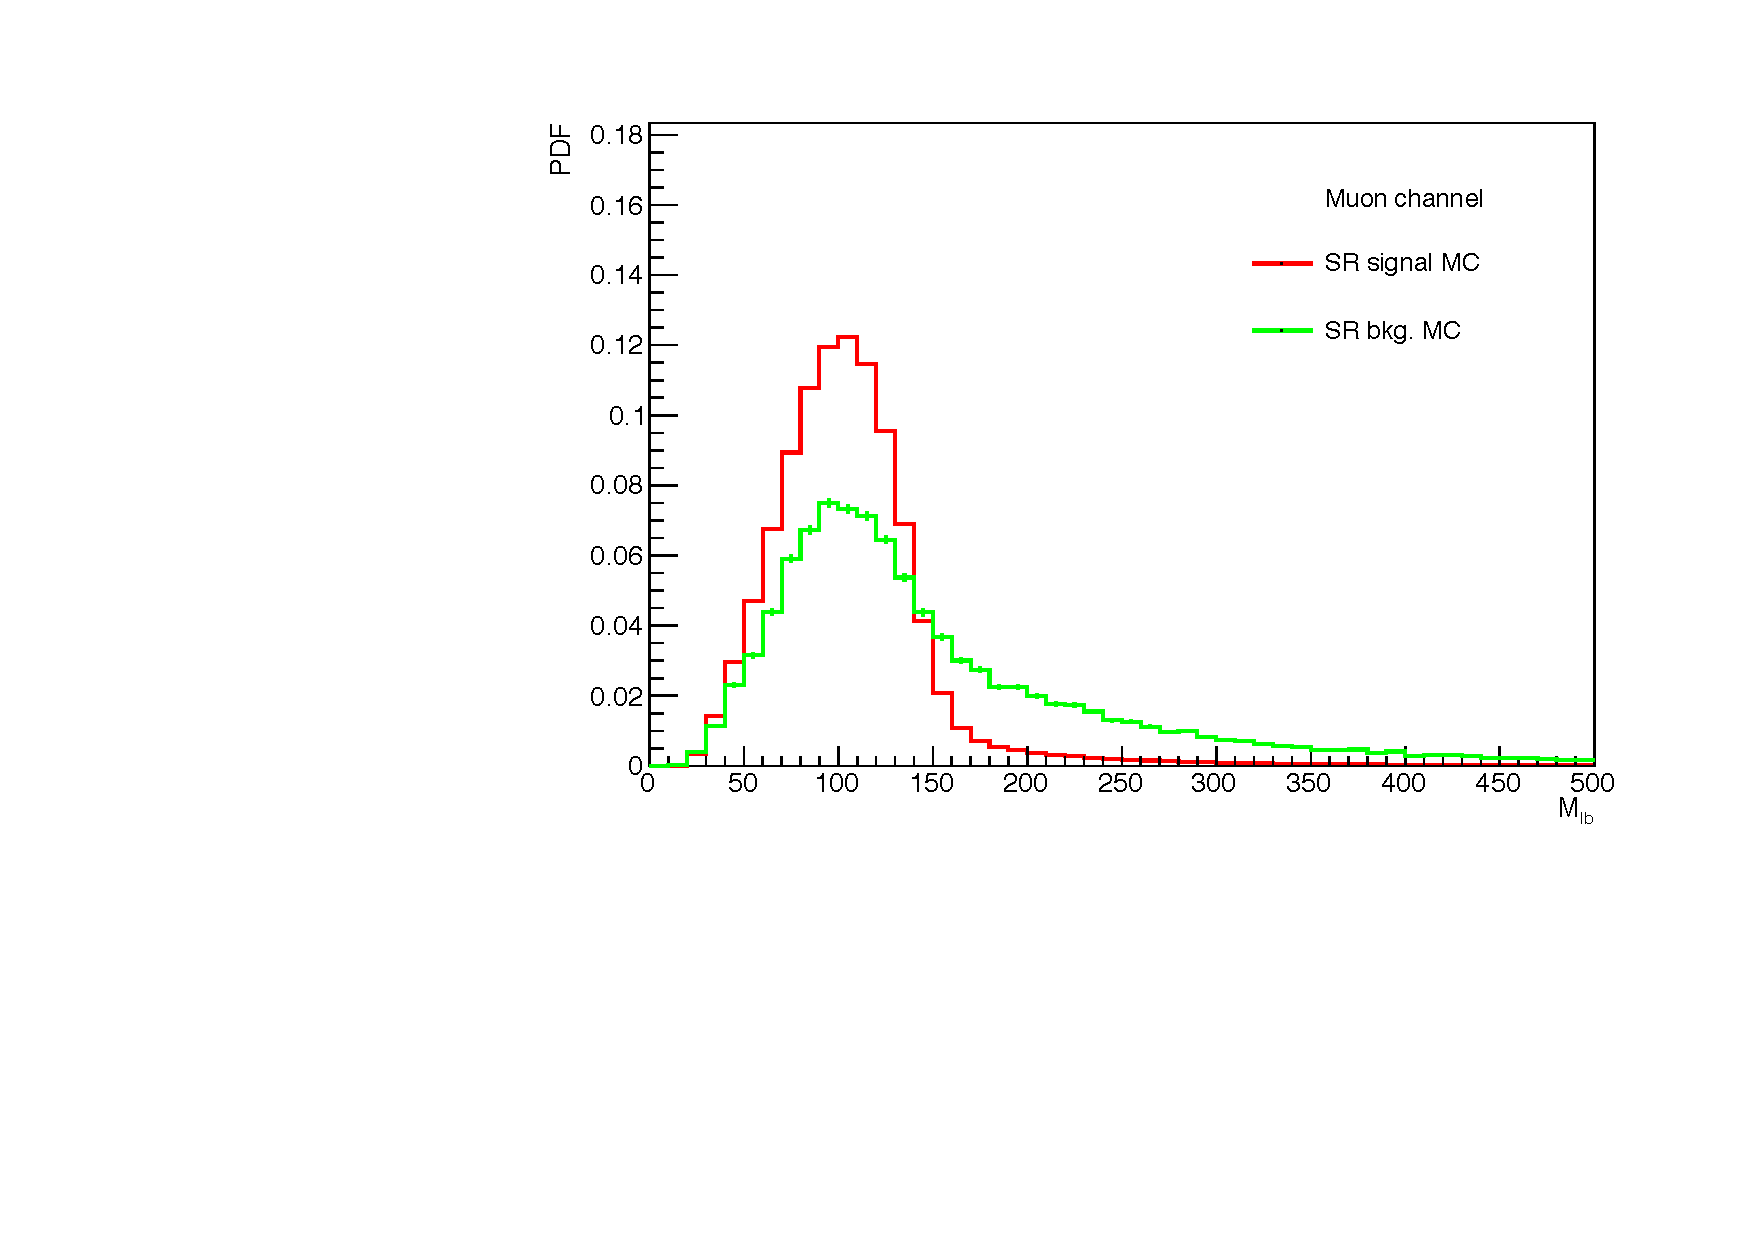
\includegraphics[width=0.45\textwidth]{Figures/BackgroundEstimation/a05_MLP_SR_sig_bkg_shape_mu.pdf}}
			\subfigure[MVA(20 variables, MLP), el-ch]{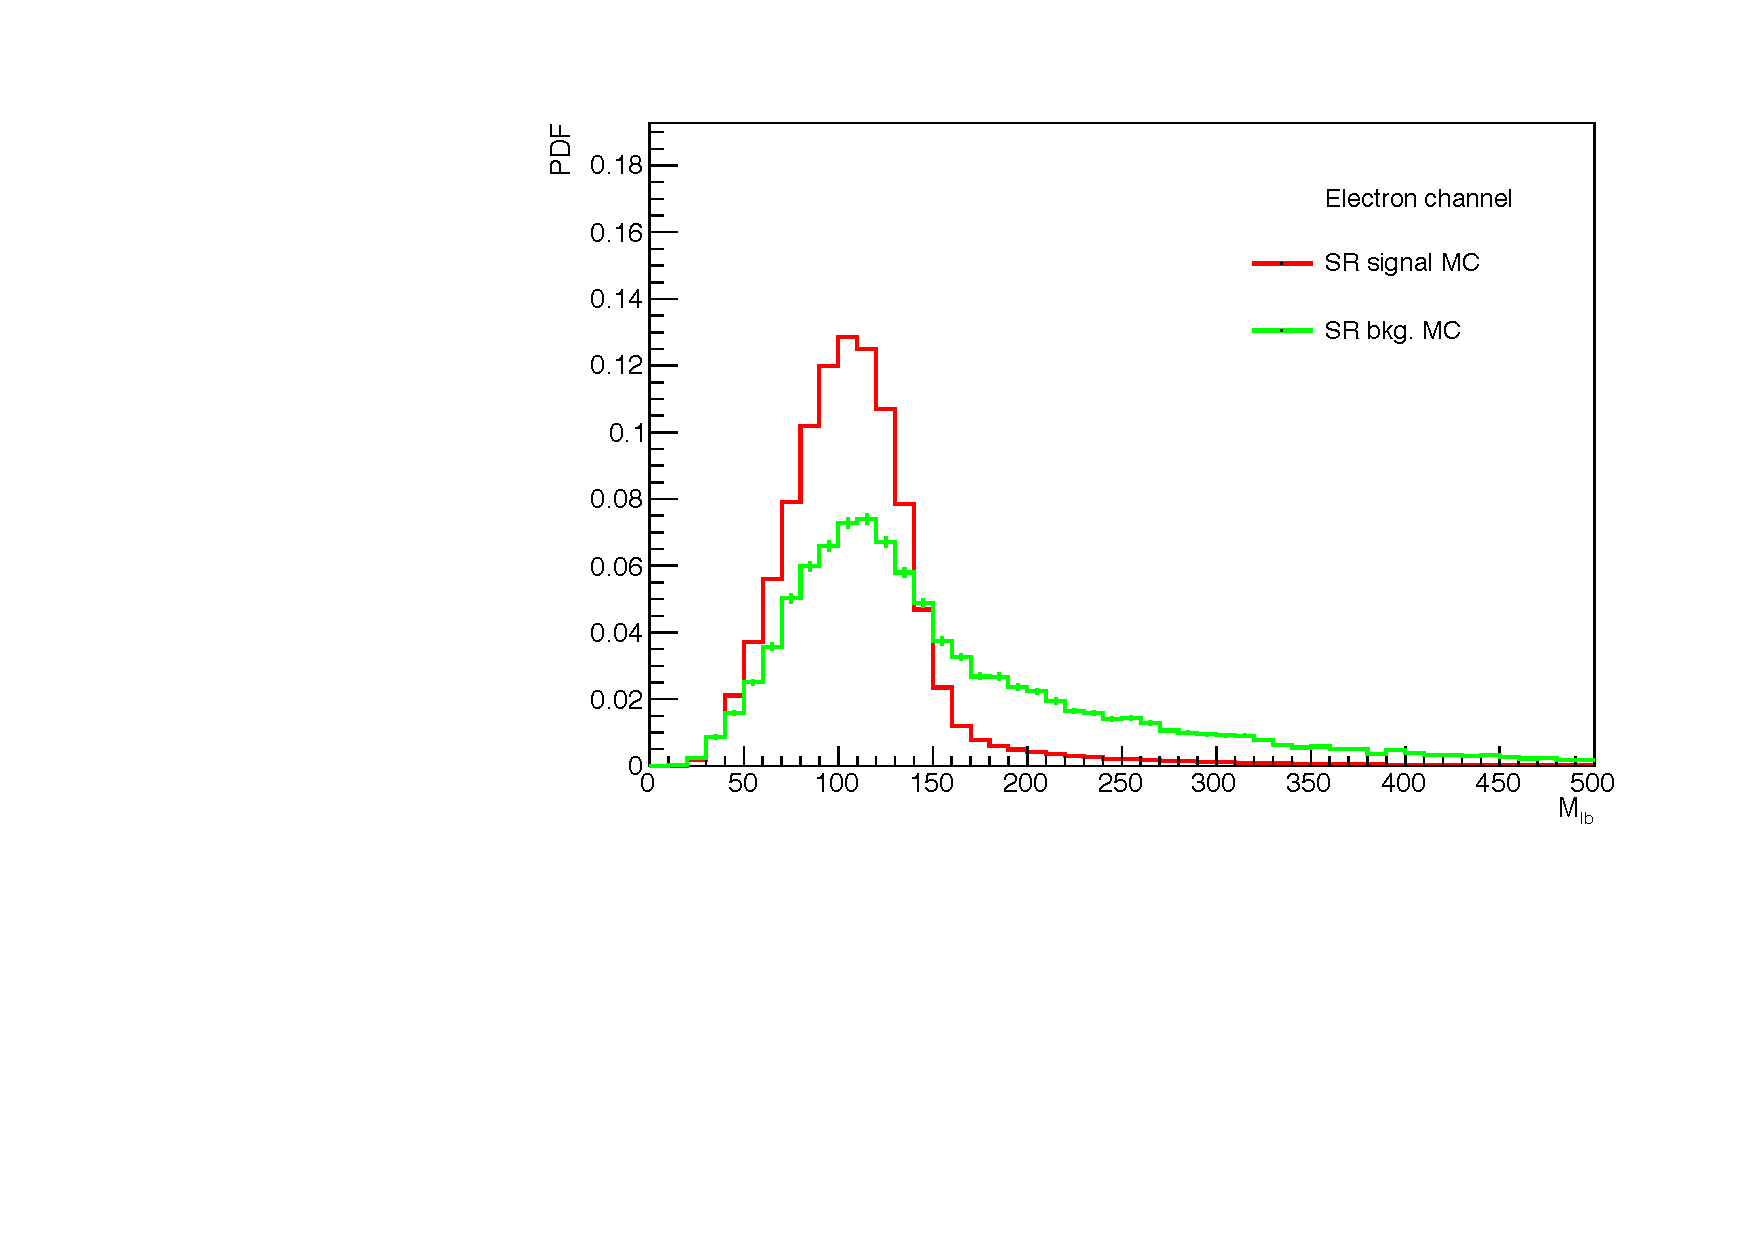
\includegraphics[width=0.45\textwidth]{Figures/BackgroundEstimation/a05_MLP_SR_sig_bkg_shape_el.pdf}}\\
		\caption{Comparison of $M_{lb}$ shape between SR's signal and background}
		\label{BkgEst:fig:SR_sigbkg_Mlbshape}
		\end{figure}
		\FloatBarrier

	\subsection{Template Fit}
	\label{ssec:TemplateFit}

		The method $\textbf{Template Fit}$ is used to estimate background yields and subtract them in this analysis. The template in this method means a pdf(probability density function) with unvaried shape under specific variable's spectrum. Also following pdf's characteristic, the template have to be normalized(integrated area of this shape is unity). This template fit is one of general fitting with $\textbf{Max-Likelihood Method}$. 

		With respect to Max-Likelihood Method, it uses the likelihood function $\emph{L}$(Eq.****) and minimizes the $-2\ln{L}$ by computing resource to get the more appropriate parameters in function we want to predict. The signal and background yields in this analysis are both the target parameters in fitting.


		There are $N$ times measurements in Max-Likelihood method. The $\{x^{i}_{1},x^{i}_{2},\ldots,x^{i}_{n}\}$ in Eq.**** is the the set of variable for $i$-th measurement.



		As mentioned that the W+jets-dominant CR's data is used to data-driven background in SR, it must be checked that how the similarity of $M_{lb}$'s pdf shape they have:

		\begin{figure}[H]
		\centering
			\subfigure[$\chi^2_{min}$, mu-ch]{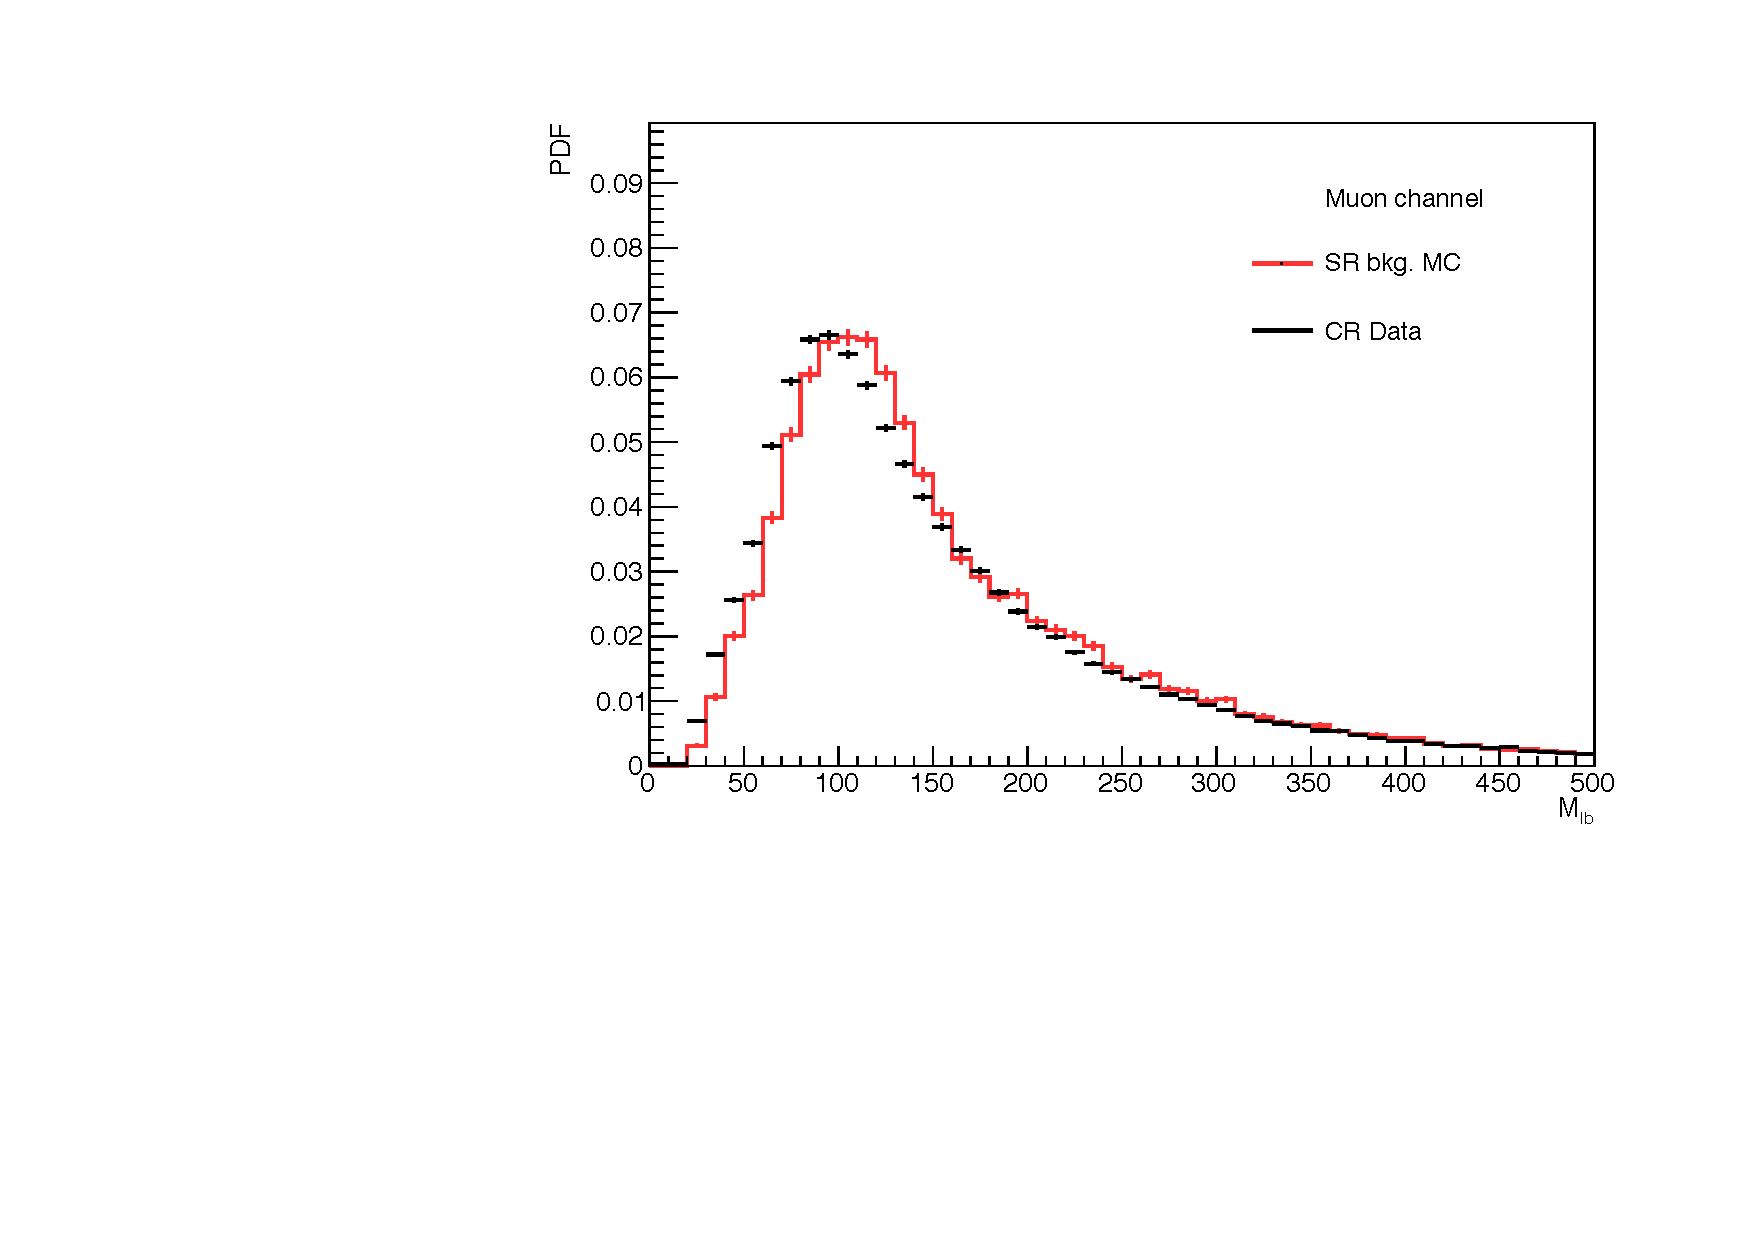
\includegraphics[width=0.45\textwidth]{Figures/BackgroundEstimation/chi2_MlbPDF_Cmp_mu.pdf}}
			\subfigure[$\chi^2_{min}$, el-ch]{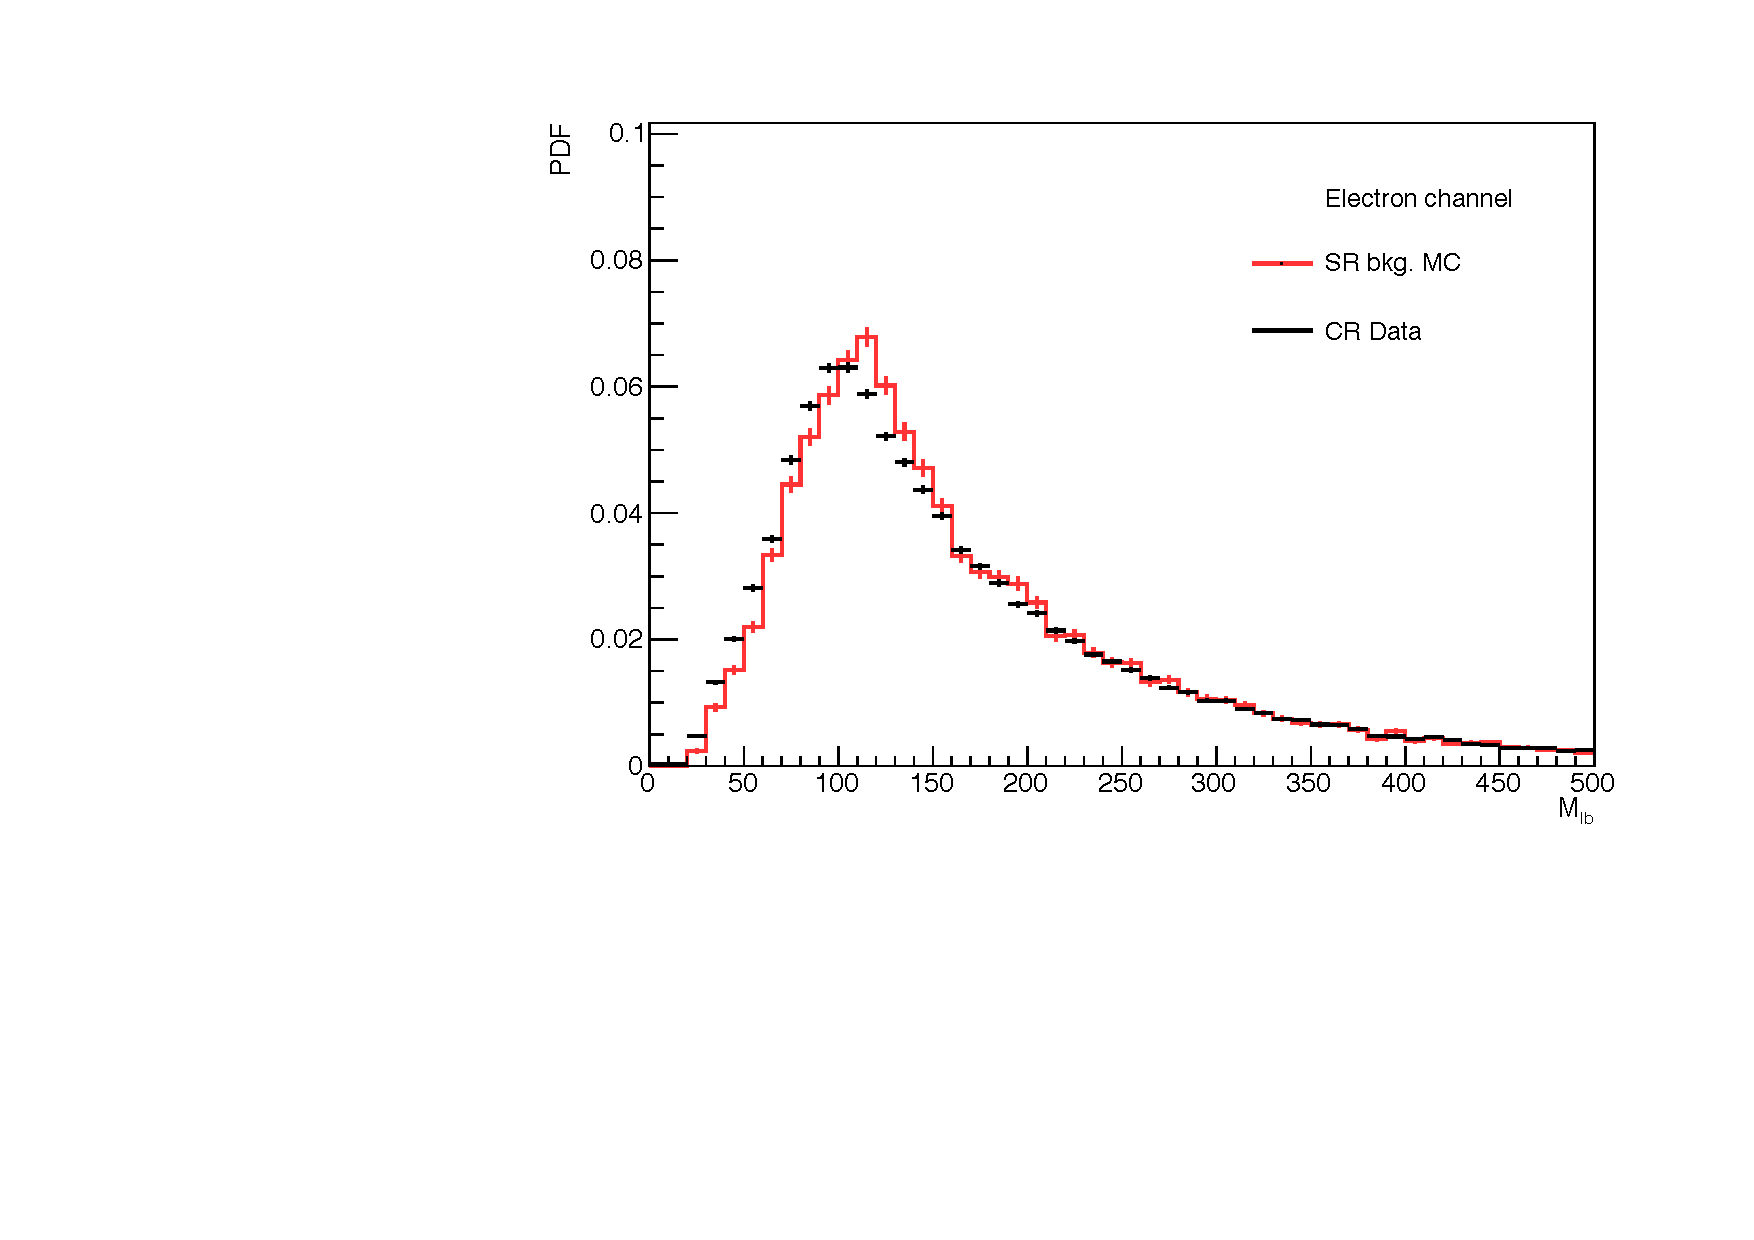
\includegraphics[width=0.45\textwidth]{Figures/BackgroundEstimation/chi2_MlbPDF_Cmp_el.pdf}}\\
		\end{figure}
		\FloatBarrier
		\begin{figure}[H]
		\centering
			\subfigure[MVA(20 variables, MLP), mu-ch]{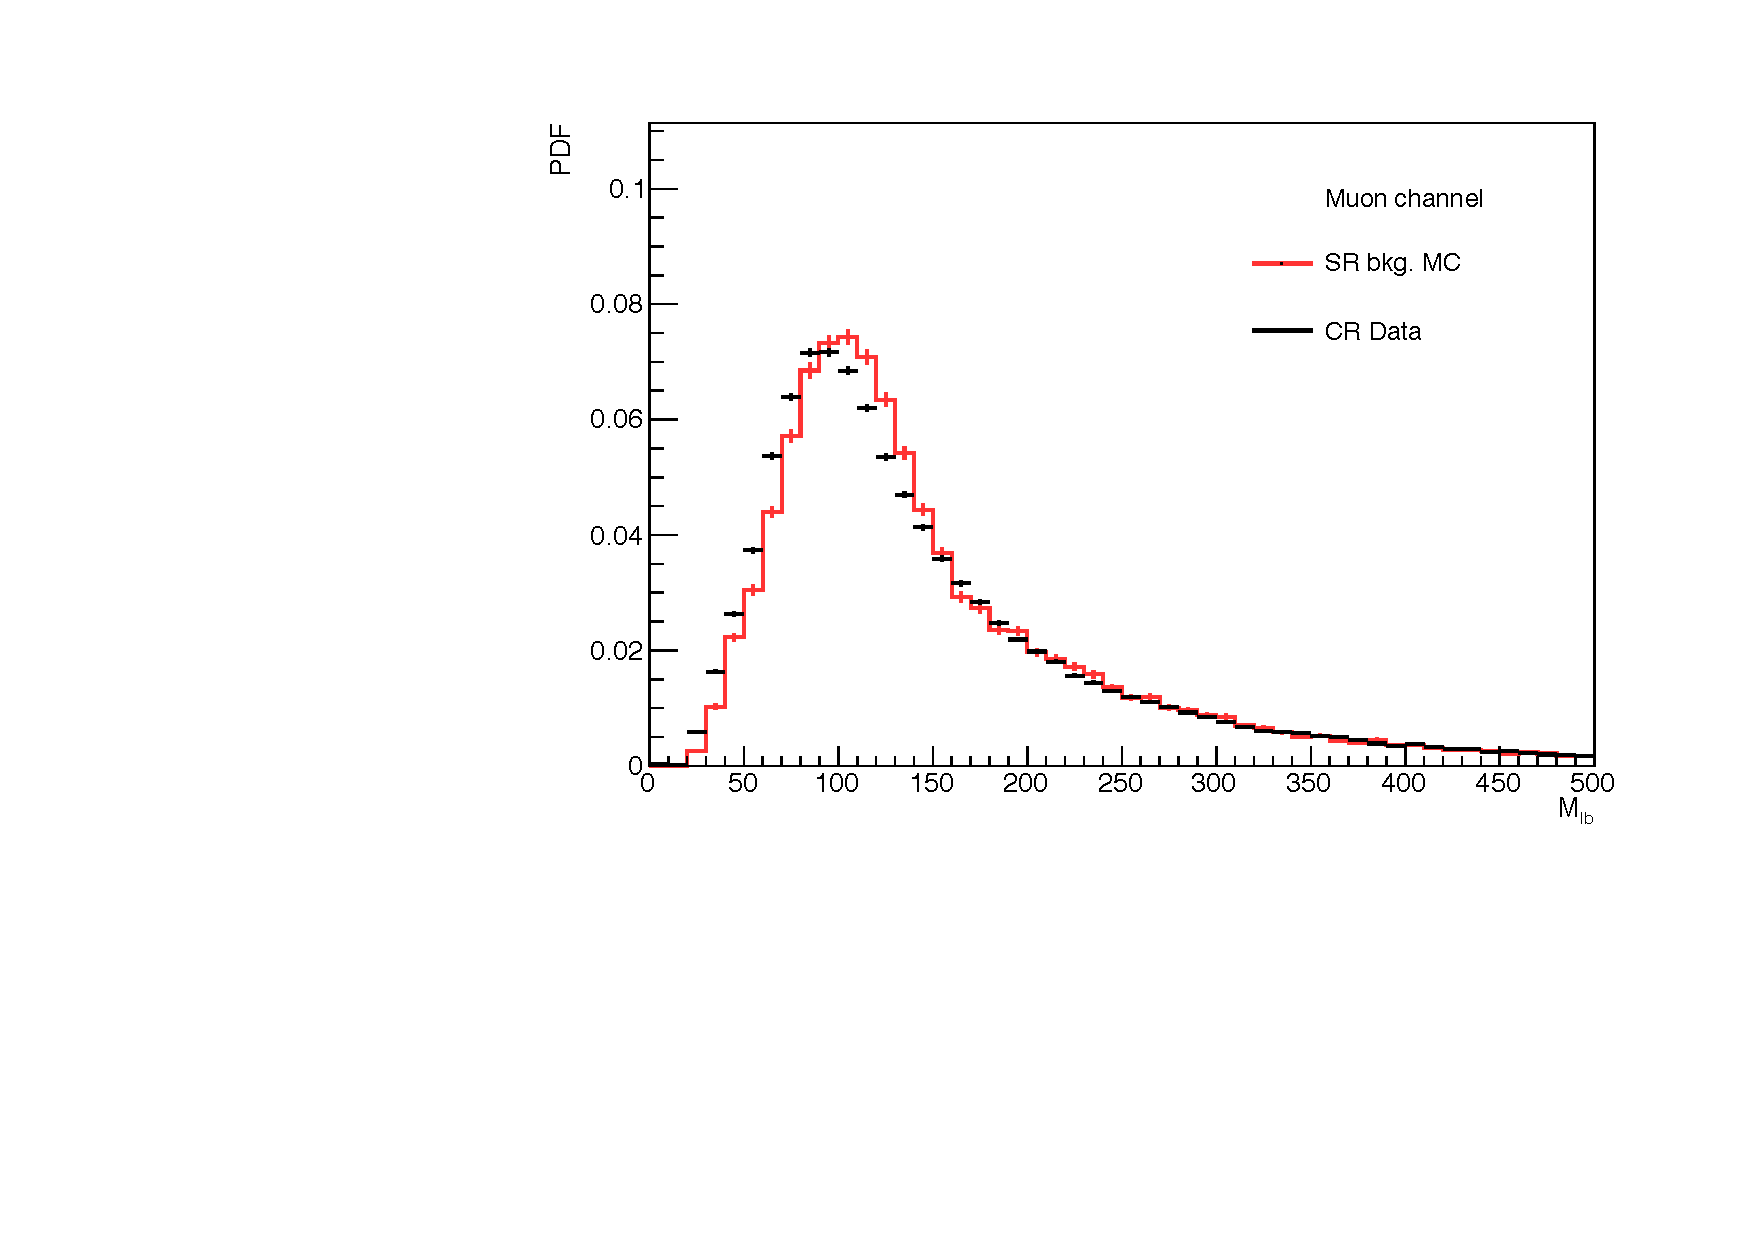
\includegraphics[width=0.45\textwidth]{Figures/BackgroundEstimation/a05_MLP_MlbPDF_Cmp_mu.pdf}}
			\subfigure[MVA(20 variables, MLP), el-ch]{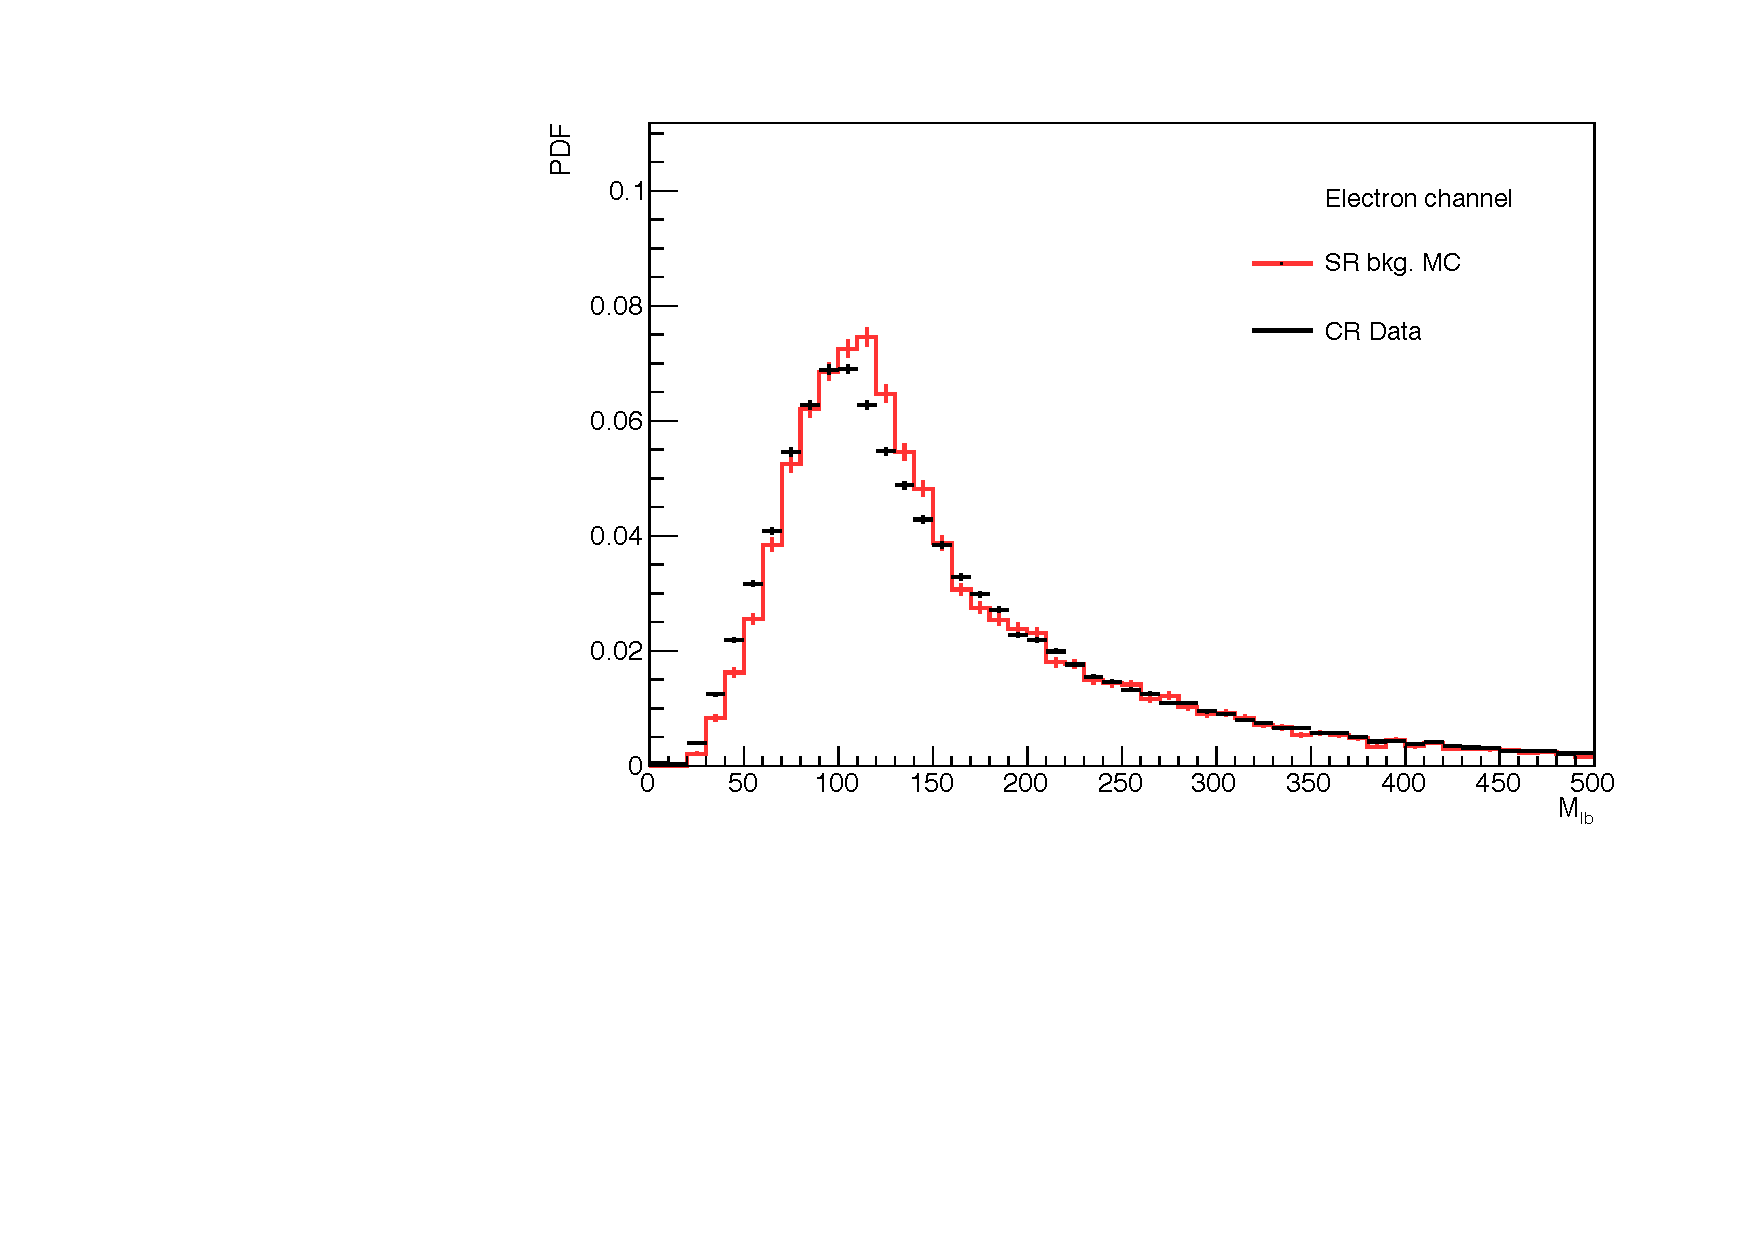
\includegraphics[width=0.45\textwidth]{Figures/BackgroundEstimation/a05_MLP_MlbPDF_Cmp_el.pdf}}\\
		\caption{Comparison of $M_{lb}$ shape between SR's background and CR's data}
		\label{BkgEst:fig:CRSR_Mlbshape}
		\end{figure}
		\FloatBarrier




		\subsubsection{Fitting Result}
		\label{sssec:FittingResult}

		\begin{center}
		\begin{longtable}[H]{ c c c }
		\caption{Data and MC estimated events number after template fit(w/ $\chi^2_{min}, M_{lb}$ cut)} \\
		\hline
		 & Muon Channel & Electron Channel \\ 
		\hline
		 Data & 243790 & 136151 \\
		\hline
		 Expected $t\bar{t}$ & 230766 & 135600 \\
		 Expected background & 12146.9 & 5537.45 \\
		\hline
		\label{BkgEst:tb:DataMC_est_chi2}
		\end{longtable}
		\end{center}
		\FloatBarrier

		\begin{center}
		\begin{longtable}[H]{ c c c }
		\caption{Data and MC estimated events number after template fit(w/ MVA-A strategy)} \\
		\hline
		 & Muon Channel & Electron Channel \\ 
		\hline
		 Data & 245436 & 139432 \\
		\hline
		 Expected $t\bar{t}$ & 236226 & 133894  \\
		 Expected background & 8520.95 & 5102.1 \\
		\hline
		\label{BkgEst:tb:DataMC_est_MVAA}
		\end{longtable}
		\end{center}
		\FloatBarrier

		\begin{center}
		\begin{longtable}[H]{ c c c }
		\caption{Data and MC estimated events number after template fit(w/ MVA-B strategy)} \\
		\hline
		 & Muon Channel & Electron Channel \\ 
		\hline
		 Data & 272583 & 157510 \\
		\hline
		 Expected $t\bar{t}$ & 256196 & 146656 \\
		 Expected background & 15479 & 10217.6 \\
		\hline
		\label{BkgEst:tb:DataMC_est_MVAB}
		\end{longtable}
		\end{center}
		\FloatBarrier

		\subsubsection{Goodness of Fit}
		\label{sssec:GoF}

	





\FloatBarrier
